%%
%% Template intro.tex
%%

\chapter{Introduction}
\label{cha:intro}
% Sequence learning. two problems. use pgm

% prob central role. directed; undirected figure1.

% pgm advantages

% directed adv

% undirected adv (efficient inference)

% explore two probs in two parts figure 2

% part1

% reinforcement learning
% kdd20: yt yt_1 yt_3

% how to use pgm solve which problem

% part2

Probabilities play a central role in sequence learning.
Probabilistic Graphical Models (PGMs)
\cite{koller2009probabilistic} provides a unified framework for
diagrammatically representing complex probability distributions
in formally defined graphs. In graph theory, a graph consists of
nodes connected by links. In PGMs, each node represents a random
variable, and the links represent probability dependencies
properties among these variables. By representing the structure
of a probability distribution in a formal graph, important
properties, such as conditional independence properties, can be
obtained by inspection of the graph. Moreover, since PGMs
establish a formal connection between probability theories and
the graph theory, computationally expensive tasks, such as
inference and learning in sophisticated models, can be solved
efficiently by employing efficient graph algorithms
\cite{Ladicky:ECCV10,Rother:CVPR09,Kohli:TR08}.

As graphs, PGMs can also be categorized into directed PGMs,
undirected PGMs and a hybrid of both (such as chain graphs
\cite{lauritzen1989graphical,frydenberg1990chain}, it contains
both undirected PGMs and directed PGMs). We illustrate PGMs of
the Hidden Markov Models \cite{eddy1996hidden} (HMMs) which is a
type of directed model, as well as Markov Random Fields
\cite{Hammersley:1971} (MRFs) which is also known as undirected
PGMs \cite{bishop:2006:PRML} in Figure \ref{fig:intro_hmm_mrf}.
Figure \ref{fig:intro_hmm_mrf} (a) denotes an HMM, in which $S$
nodes denote random variables of environment states, namely the
observed information. $Y$ nodes are random variables for latent
information. Directions of the probability dependencies are
represented by connecting links' directions. In this graph, $S$
nodes are sequentially dependent on parent nodes. $Y$ nodes only
depend on corresponding $S$ nodes at the same time step. Figure
\ref{fig:intro_hmm_mrf} (b) denotes a MRF, each node in this
graph represents a random variable of an entity (such as a city).
Directions of probability dependencies in this model is
unspecified: directions of information flows are complex and keep
changing over time.
\begin{figure*}[h]
  \centering
  \begin{tabular}{cc}
    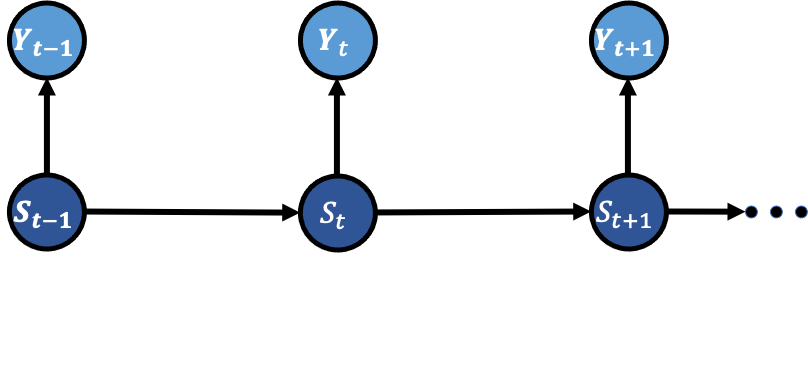
\includegraphics[width=0.5\linewidth]{figures/HMM.png} &
                                                             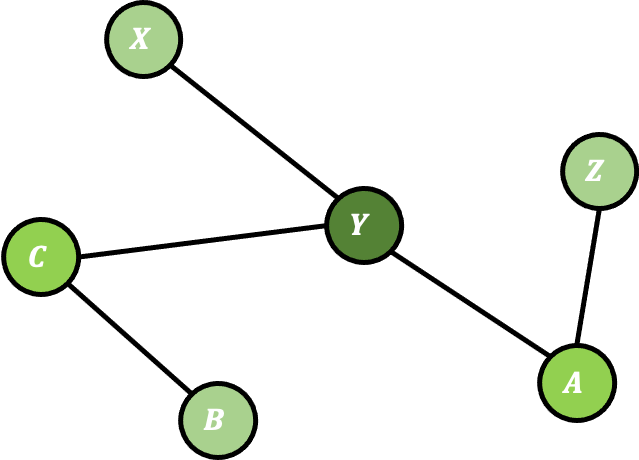
\includegraphics[width=0.4\linewidth]{figures/MRF.png}\\
    {\small (a) HMMs: Directed PGMs}& {\small (b) MRFs: Undirected PGMs}\\
  \end{tabular}
  \caption{\label{fig:intro_hmm_mrf} Illustration of PGMs. Figure
    (a) is the PGM of Hidden Markov Models (HMMs), a type of
    directed graph. Directed links between nodes represent
    conditional independences in the probability distribution.
    Figure (b) is the PGM of Markov Random Fields (MRFs), a type
    of undirected graph. Each node denotes a random variable.
    Nodes are connected to each other with arbitrarily many
    undirected connections.}
\end{figure*}

In this thesis, we demonstrate rarely discussed sequence learning
challenges by exploiting both directed and undirected PGMs'
advantages. The probabilistic description of sequences (such as
time series, DNA sequences etc.) has been a long standing
problem. Initially, researchers made strong assumptions, such as
sequences are independent and have identical (following the same)
probability distributions
\cite{bachelier1900theorie,friedman1953methodology}. Assumptions
like these have effectively simplified the complexity of modeling
sequences' dynamics and quickly became the foundation of many
predominant machine learning, engineering and finance theories
\cite{jegadeesh1993returns,shiller1980stock,
  sharpe1964capital,carhart1997persistence,sargent1993bounded}.
Despite the significant successfulness of previous researches,
researchers have found many major discrepancies between those
strong assumptions and real world problems
\cite{lux2008markov,mandelbrot1963new,lux2007forecasting,
  abry2019shuffling, li2019multi, mandelbrot1997multifractal}.
These long standing challenges mainly fall into three categories:
%
\begin{enumerate}
\item Heterogeneous (Non-stationary) distributions (of a single
  sequence). Dependency relationships (\eg transition probability
  distributions of a Markov chain etc.) keep changing over time
  \cite{ross1996stochastic}.
\item Multi-timescale (Multi-scale) information dependency (of a
  single sequence). Even for a single sequence, information
  encoded in long and short time scale are inter-dependent.
  Information extracted from a single time scale is incomplete
  \cite{mandelbrot1997multifractal}.
\item Higher-order (greater than or equal to 3) dynamics (of
  multi-sequences). Most sequences not only have dependencies on
  themselves. They are also strongly affected by other correlated
  sequences and have complex dynamics (\eg directions of
  information flow keep changing over time) dependencies with
  them
  \cite{lo1990contrarian,badrinath1995shepherds,mcqueen1996delayed}.
\end{enumerate}
%
In this thesis, we relax conventional assumptions, such as the
$i.i.d$ (independent and identically distributed) assumption, on
sequences and demonstrate challenges above under the
Probabilistic Graphical Models (PGMs) framework. Among three
challenges, the first heterogeneous assumption is the most
general assumption, and has to be treated differently while
addressing the second and third challenges. Therefore, we split
this thesis into two parts. Part \ref{part:1} addresses the
multi-timescale challenge by using directed PGMs under the
Reinforcement Learning paradigm. Part \ref{part:2} addresses
the higher-order dynamics challenge by using undirected PGMs
under the Supervised Learning paradigm. Both two parts are under
the heterogeneous assumption. The arrangement of this thesis is
shown in Figure \ref{fig:intro_content}.
\begin{figure*}[h]
  \centering
  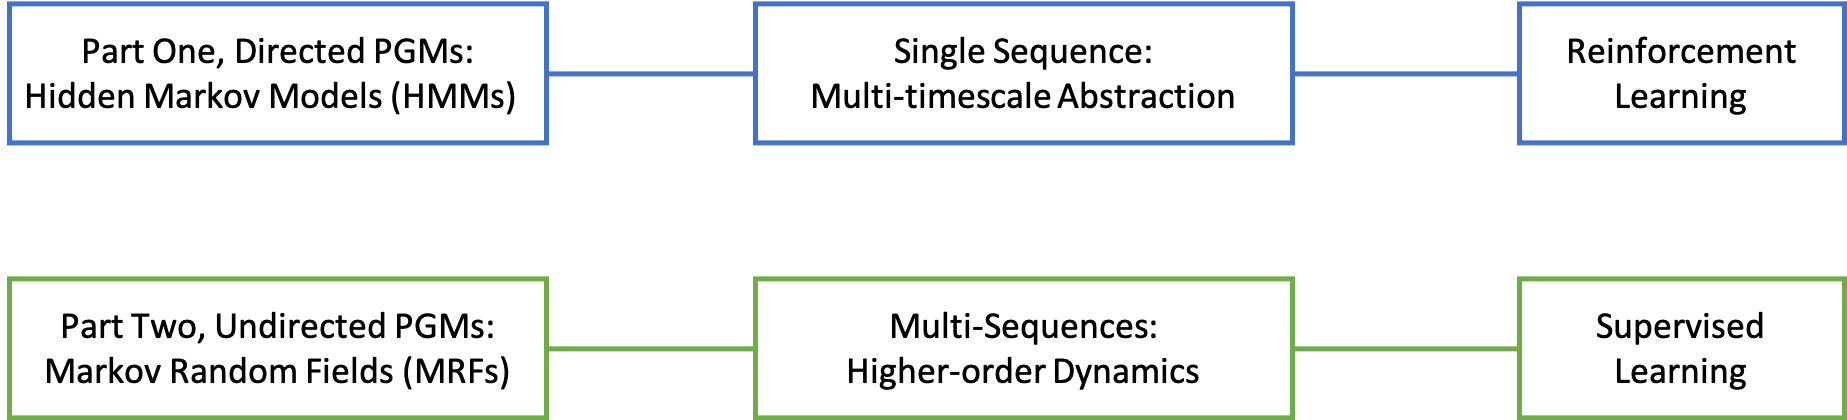
\includegraphics[width=1\linewidth]{figures/content.png}\\
  \caption{\label{fig:intro_content} Thesis Arrangement. Part
    \ref{part:1} focuses on learning one single sequence.
    Multi-timescale information is abstracted by Hidden Markov
    Models (HMMs) under the Reinforcement Learning paradigm. Part
    \ref{part:2} focuses on learning dynamics between groups of
    sequences. Dynamics among higher-order groups (any group
    contains greater or equal to three entities) of sequences is
    captured by Markov Random Fields (MRFs) under the Supervised
    Learning paradigm.}
\end{figure*}

Part \ref{part:1} focuses on demonstrating the multi-timescale
challenge \cite{mandelbrot1997multifractal} on a single sequence.
The multi-timescale, or more generally, multi-scale problem
presents a common phenomenon that information on different scales
of the same entity are inter-dependent: they are interwoven in
both micro and macro scales. In order to understand the sequence,
information encoded in different scales must be considered
simultaneously: details are lost when the attention is only paid
to the macro scale, while the big picture is overlooked when only
the micro scale is paid attention to. This phenomenon does not
only restrict to temporal sequences, it also applies to other
sequences such as natural languages and even images. We
illustrate this idea in Figure \ref{fig:intro_fractal}. However,
in this thesis we mainly use temporal sequences for experiments
and use the term ``multi-timescale'' over ``multi-scale'' for
explicitness.

\begin{figure*}[h]
  \centering
  \begin{tabular}{cc}
    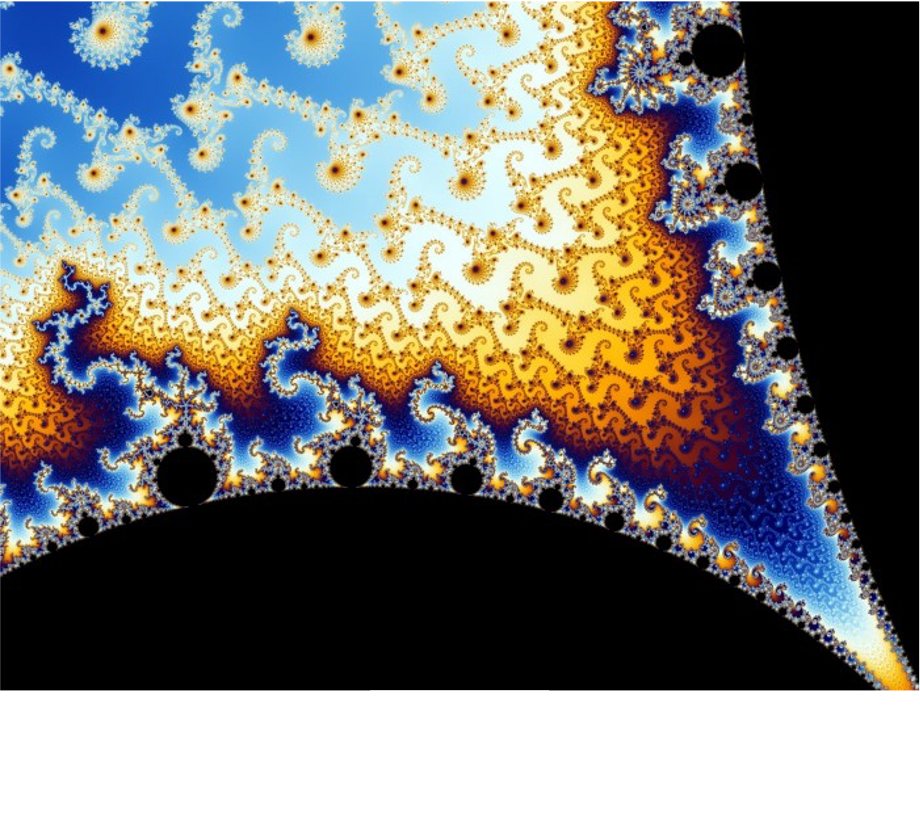
\includegraphics[width=0.35\linewidth]{figures/fractal.png}
    &
      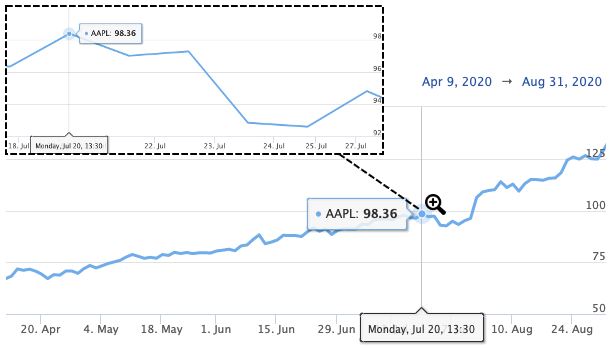
\includegraphics[width=0.65\linewidth]{figures/stock.png}\\
    {\small (a) Mandelbrot Set}& {\small (b) Stock Price}\\
  \end{tabular}
  \caption{\label{fig:intro_fractal} Illustration of the
    multi-scale assumption. Figure (a) is the famous Mandelbrot
    fractal. It is grown by starting from the smallest basic
    shape and keep repeating itself at larger scales. The
    information encoded in micro scale can not be overlooked
    since it determines the macro scale. On the contrary, Figure
    (b) is the stock price of the Apple company. It is misleading
    if only the downside micro scale (up-left zoomed-in period)
    is paid attention to, because at a macro scale the Apple
    stock is at a long-term upside. Therefore, even on a single
    sequence, information encoded in multi-scale must be paid
    attention to simultaneously.}
\end{figure*}

To address the multi-timescale challenge,
\citename{mandelbrot1997multifractal} made a ground-breaking
contribution by introducing multi-fractal probability
distributions into sequence learning. A multi-fractal
distribution is proposed to approximate multi-timescale sequences
with ground-truth labels under the Supervised Learning paradigm.
However, the self-similarity constraint (different time scales
follow the same distribution) made by the multi-fractal
distribution is a strong assumption and only applies to a small
subset of multi-timescale sequences. Also, the problem of
multi-timescale dependencies goes beyond the Supervised Learning
paradigm. In Supervised Learning, the term of ground-truth labels
are fixed: most existing methods choose $y_{t+N}$ as a regression
target for inputs $\mX_t$ at time step $t$ where $N$ is a
constant. Such assumption no longer holds under the
multi-timescale dependence assumption because $N$ becomes a
variable rather than a constant. $\mX_t$ can be responsible for
generating $y_{t+?}$ any time earlier or later than the
fixed-term $N$. This makes Reinforcement Learning
\cite{sutton2018reinforcement} (RL), a framework which does not
require ground-truth labels and learns from interactions with the
environment, the perfect paradigm for modeling multi-timescale
sequences.

Reinforcement Learning (RL) is a paradigm for imitating humans'
trial-and-error learning process. In RL, there is no ``correct
answers'' (labels) as in Supervised Learning. RL trains an agent
to maximise the expectation of all incoming future rewards by
taking actions in and receiving feedback from an environment.
Therefore, the RL paradigm does not suffer from the fixed-term
labeling problem as the Supervised Learning does. RL has achieved
human-level performance in playing video and board games
\cite{mnih2015human,silver2016mastering}. However, conventional
RL agents have limited abilities to solve complex tasks
\cite{daniel2016probabilistic}: they only learn the most
primitive actions and make decisions at the smallest time scale.
Hierarchical Reinforcement Learning (HRL) attempts to resolve
this gap between humans and RL by decomposing complex tasks into
a hierarchy of abstracted actions at multiple time scales. An HRL
agent typically learns abstractions of actions on two levels:
skills and primary actions. Skills are higher-level abstracted
actions. Their executions are temporally extended to a variable
amount of time. Primary actions are lower-level actions defined
by the environment. They are executed at every time step. For
example, for a humanoid robot, walking and jumping are two
abstract skills, while movements of each joint are primary
actions. The main contribution of Part \ref{part:1} focuses on
solving the first two challenges together by employing the option
framework \cite{sutton1999between}, one of the most promising HRL
frameworks.

The option framework is developed based on the Semi-Markov
Decision Problem (SMDP). There are, however, four inherent
problems: the option framework 1) has low sample efficiency, 2)
cannot employ more stable Markov Decision Problem (MDP) based
learning algorithms, 3) represents abstract actions implicitly,
and 4) is expensive to scale. To overcome these shortcomings, in
\Chapref{cha:sa}, we propose a simple yet effective MDP
implementation of the option framework: the Skill-Action (SA)
architecture. Derived from our novel discovery that the SMDP
option framework has an MDP equivalence, SA hierarchically
extracts skills (abstract actions) from primary actions and
explicitly encodes this knowledge into skill context vectors
(embedding vectors). Although SA is MDP formulated, skills can
still be temporally extended by applying the attention mechanism
to skill context vectors. Under this formulation, SA can be
optimized with any MDP-based policy gradient algorithm, it is
also sample efficient, inexpensive to scale, and theoretically
proven to have lower variance than other frameworks. Our
empirical studies in \Chapref{cha:sa_app} on challenging infinite
horizon robot simulation environments demonstrate that SA not
only significantly outperforms all baselines, but also exhibits
smaller variance, faster convergence, and high interpretability.
SA also outperforms the other models on transfer learning tasks
and demonstrates its advantage in knowledge reuse tasks. SA has
the potential to pave the way for a large scale pre-training
architecture in reinforcement learning.

Part \ref{part:2} addresses the higher-order dynamics between
multiple sequences by using undirected PGMs under the Supervised
Learning paradigm. Most existing sequence learning literatures
\cite{sargent1993bounded,jegadeesh1993returns,shiller1980stock,
  carhart1997persistence,lux2007forecasting,lux2008markov,abry2019shuffling}
only consider how to model a single sequences' dynamic. Rare
literatures investigate how correlated sequences evolve together
and the complex dynamics between them. Modeling dynamics between
higher-order (greater than or equal to three) sequences is very
challenging. This is because directions of information flow
between sequences (entities) are usually unobserved and keep
changing over time.

\begin{figure*}[h]
  \centering
  \begin{tabular}{cc}
    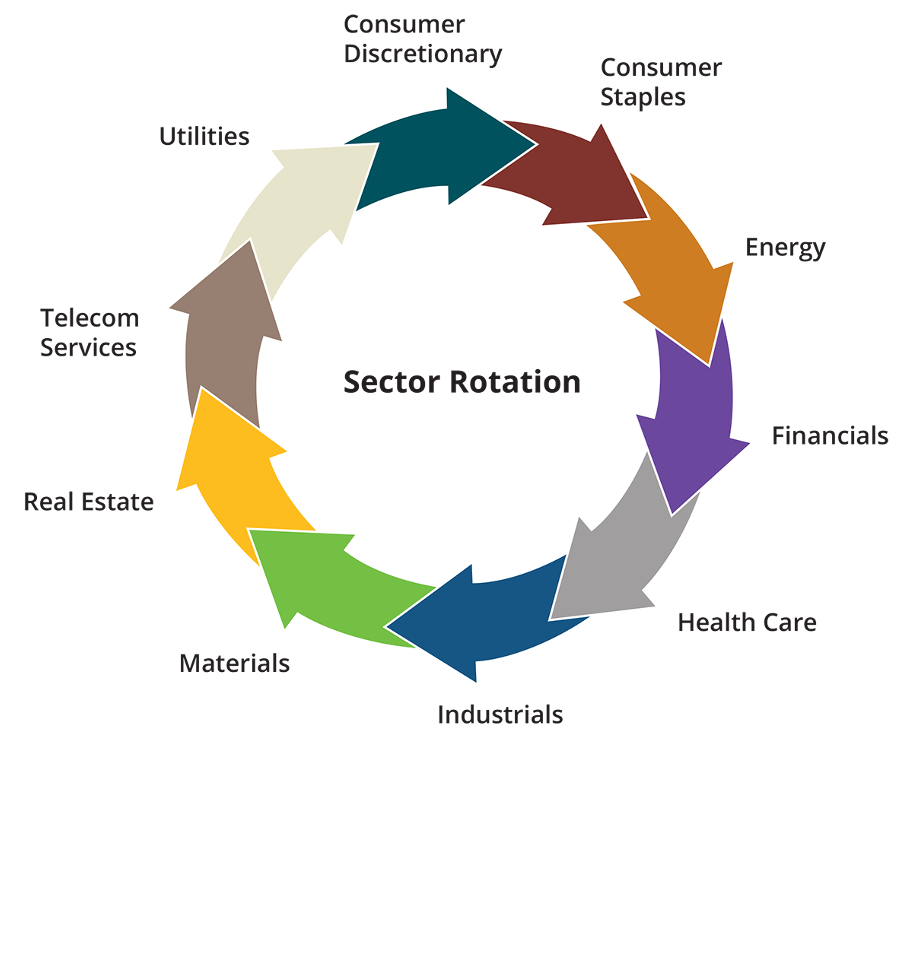
\includegraphics[width=0.3\linewidth]{figures/intro_sector.png}
    &
      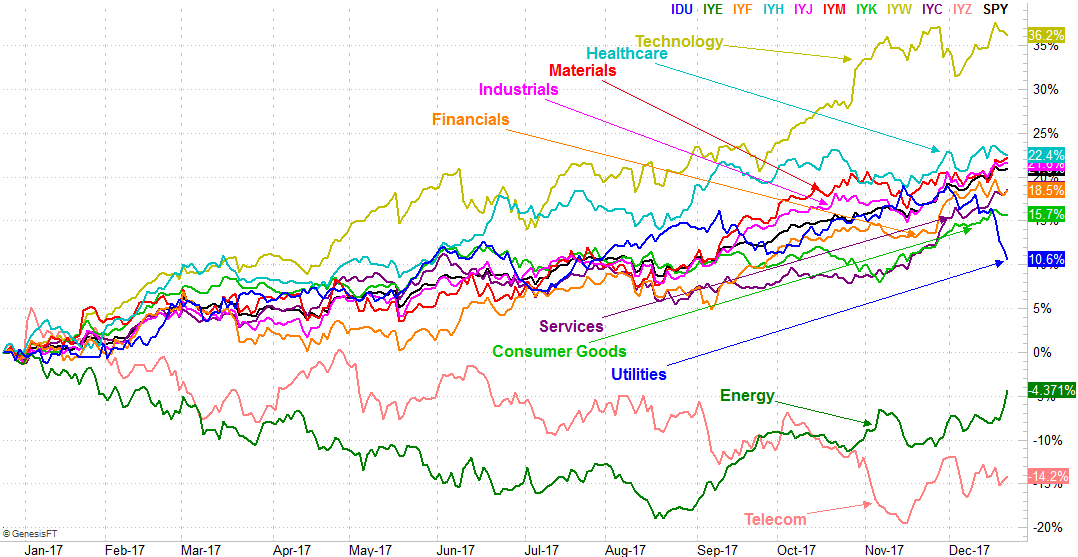
\includegraphics[width=0.7\linewidth]{figures/intro_rotation_price.png}\\
    {\small (a) Sector Rotation}& {\small (b) Sector Price}\\
  \end{tabular}
  \caption{\label{fig:intro_fractal} Illustration of the
    higher-order dynamics in the economy. Figure (a) illustrates
    several important sectors in the economy, such as real
    estate, industrials, utilities, materials, and energy. These
    sectors are building blocks of the economy and each sector's
    growth not only depends on itself but other sectors. Figure
    (b) shows the actual U.S. Sectors Indices in year 2017. As
    shown in the Figure. Most sectors are positively correlated
    at a macro scale while have many exceptions at a micro scale.
    These kind of dependences are too complex to be represented
    as directed PGMs and can only be learned from data by
    undirected PGMs.}
\end{figure*}

The most well known example is how the economy grows. As shown in
Figure \ref{fig:intro_fractal}, the gross economy is constituted
of many sectors, such as real estate, industrials, utilities,
materials, and energy. All these sectors are closely correlated
and evolves together. If the gross economy is a graph, these
sectors are the nodes and are all linked together. However, the
dependence relationships between these sectors are too complex to
be expressed as directed PGMs: as shown in Figure
\ref{fig:intro_fractal} (b), their dependences keep changing over
time
\cite{lo1990contrarian,mech1993portfolio,brennan1993investment}.
Using the energy and telecommunications sectors as an example,
during most of the time in 2017 these two sectors are positively
correlated. However, between September and November, these two
sectors evolves in opposite directions. Therefore, dynamics
between higher-order sequences are too complex to be expressed as
directed PGMs and have to be learned from data by exploiting
undirected PGMs.

Markov Random Fields (MRFs), also known as undirected
Probabilistic Graphical Models (PGMs) \cite{bishop:2006:PRML},
are as simple as regularized joint probability distributions. One
specialty of MRFs is that they are factorized over (conditional
independent on) maximal cliques (such as sectors, more details
in~\Secref{sec:MRF}) of random variables defined on the
undirected graph. In many applications, structural information,
such as sub-objects to the whole object relationships and
relationships between sub-objects, can be well represented in
maximal cliques. By defining each maximal clique's probability
distribution and optimizing over them, MRFs provide a powerful
framework for modeling complex higher-order dynamics between
entities. However, the advantages of MRFs are limited by its
computational complexity. Many literatures
\cite{Kohli:TR08,pletscher2012learning,Ladicky:ECCV10,Szummer:ECCV08}
found that although MRFs are able to represent a rich class of
higher-order dynamics, only a small set of them are
computationally feasible \cite{gouldlearning,Park:ECCV2012}.

To exploit MRFs advantages on encoding higher-order dynamics and
address the computational efficiency problem, in
\Chapref{cha:mrf}, we propose a novel and powerful MRF-LSSVMs
framework. We first prove that binary MRFs with Lower Linear
Envelope Potentials (LLEPs), a type of higher-order potentials,
have an equivalent pseudo-boolean \cite{Boros:MATH02}
formulation. Based on this equivalence, we prove the sub-modular
property of MRFs. The sub-modular property enables us to develop
an efficient inference algorithm based on the graph-cuts
algorithm \cite{Kolmogorov:PAMI04}. As for the learning
algorithm, we prove that MRFs with LLEPs can also be written in a
novel formulation which is a linear combination of parameters and
feature vectors with latent variables. Therefore, this novel
formulation establishes a connection between higher-order MRFs
and the Latent Structural Support Vector Machines (LSSVMs)
\cite{yu2009learning}. By employing the LSSVMs, we can solve the
learning problem efficiently under LSSVMs' large margin framework
\cite{tsochantaridis2005large}. In \Chapref{cha:mrf_lssvm_app},
we continue our experiment on the real financial market stock
price data set and show how MRF-LSSVMs can be used to model
dependency dynamics between time series. In order to do that, we
first employ Recurrent Neural Networks (RNNs) as unary energy
functions. Each stock is treated as a unary node in MRFs and RNNs
are used to extract feature from each stock's historical market
price time series. We then layer MRFs on top of RNNs extractor
and optimize the entire framework with the LSSVMs algorithm
proposed in \Secref{sec:opt}.

The objective of this thesis is to demonstrate three challenges
in sequence learning as mentioned above. The thesis consists of
two parts. Part \ref{part:1} addresses the multi-timescale
challenge by using directed PGMs under the Reinforcement Learning
paradigm. In \Chapref{cha:sa}, we propose a simple yet effective
the Skill-Action (SA) architecture, to model multi-timescale
sequences based on Markov Decision Problems (MDPs). We also
develop the optimization framework for SA under the Hierarchical
Reinforcement Learning (HRL) paradigm. In \Chapref{cha:sa_app},
we conduct experiments of SA on challenging robots simulation
environments and demonstrate the effectiveness of SA. Part
\ref{part:2} addresses the higher-order dynamics challenge by
using undirected PGMs under the Supervised Learning paradigm. In
\Chapref{cha:mrf}, we propose the novel MRF-LSSVMs to model
higher-order dynamics. We propose an exact inference algorithm
based on the graph-cuts algorithm for binary Markov Random Fields
(MRFs) and solve the learning problem under the efficient Latent
Structural Support Vector Machines (LSSVMs) framework. In
\Chapref{cha:mrf_lssvm_app}, we adapt MRF-LSSVMs on the financial
time series by employing Recurrent Neural Networks (RNNs) as
feature extractors and demonstrate the effectiveness of our
framework on the challenging China Securities Index (CSI) 300
data set.

%%% Local Variables: 
%%% mode: latex
%%% TeX-master: "thesis"
%%% End: 
